\chapter{Theoretical Background}\label{chap:theorBack}


\section{Basic Concepts of Machine Learning}
Machine Learning is a subject of Computer Science that studies the development of mathematical formulations that allows software to learn autonomously, without an explicit description of each rule of operation. Its goal is to extract latent characteristic features in datasets that allow an immediate classification of each input data into a particular class -- the catch is that there is no previous rule formulation, but instead we have an adaptive model that adjusts is parameters automatically from the input data it receives. 

Let us consider a practical example. For instance, suppose we want to build a device that given an input audio waveform representation of a spoken word, it matches it into a particular word of a dictionary. We could, of course, devise a set of rules and exceptions for each word analysing some of its features (perhaps the Fourier representation of each one, and, from it, manually finding the appropriate rules for each), but apart from it being a very complex task, it wouldn't be a scalable solution, given the enormous number of words in each language. The approach taken by Machine Learning is diametrically different, and instead of manually processing each waveform, we build a large dataset, of size $N$, containing the waveforms of several words $\left[ \mb{x}_1 \; \mb{x}_2 \;\mb{x}_2 \; \dots \mb{x}_N \right]$ -- we call this dataset the \textbf{training dataset} -- and we feed it to our model. Each of the $i$-th data point was previously labelled, and in fact we feed each training data point $\mb{x}_i$ \emph{along} with its corresponding label $t_i$, so that the model can adapt its parameters accordingly to the \emph{target value} it is supposed to classify. This set of labels $\mb{t} = \left[ t_1 \; t_2 \; t_3 \; \dots \; t_N \right]$ is called the \textbf{target vector}. 

We are, then, left with the following question: how can the model quantitatively evaluate the quality of its current set of parameters? That could be achieved in a number of ways, but the most usual is using a \textbf{Cost Function} that, as the name suggests, measures the cost of each wrong classification of the model. The model then evolves in a way that minimizes the cost function. A usual choice for the cost function is the \textbf{sum of squares error}. Mathematically, if $y_{\theta}^i = y_{\theta}(x_i)$ is the prediction for the input data point $x_i$ with label $t_i$, given the current set of parameters $\theta$, the cost function using this metric is given by

\begin{equation}\label{eq:costfunctionFund}
	J(\theta) = \frac{1}{2} \sum_{i=1}^N \left( y_{\theta}^i - t_i \right)^2.
\end{equation}

Furthermore, sometimes instead of applying the raw data to the model, we can apply some sort of preprocessing to the data to extract the relevant features from it. For instance, instead of just feeding a raw image, we can perform several operations like edge detection, and apply them in parallel.

The problems described above are, in fact, a subset of the problems that Machine Learning tries to address. These problems are called \textbf{classification problems}, because for each input data point, our model tries to fit it into the most appropriate class. But we can also address \textbf{regression problems} where the output is not limited to a discrete set of values but rather a continuous interval. 

In summary, the most typical setting for a Machine Learning problem is having a large \textit{input dataset} which we use to \textit{train} our model (i.e. allowing him to dynamically adapt its set of parameters $\theta$), in order to produce an output label $y_i$ for each of them that minimizes a quality metric, typically defined as a \textit{cost function}. Artificial Neural Networks are one of the tools used in Machine Learning to perform this task, and will be discussed in Section~\ref{sec:theorBack_ann} as somewhat of a contextual introduction to the main theme of the thesis, which will be Recurrent Neural Networks (Section~\ref{sec:theorBack_rnn}), namely the \textbf{Long Short-Term Memory Networks} (Section~\ref{sec:theorBack_lstm}). These two last networks branch even further from these set of problems, and are usually employed in \textit{Deep Learning} tasks, where we try to extract even higher level information from data at the expense of increased model complexity. 

\section{Artificial Neural Networks}\label{sec:theorBack_ann}

Artificial Neural Networks (ANN) are mathematical structures that, as the name suggests, try to mimic the Human Brain. ANN's building blocks, like their biological counterpart, model the high-level behaviour of biological neurons, in the sense that they neglect unnecessary biological aspects (such as modeling all the voltages across the neuron and all its electromagnetic interactions), and only retain its fundamental underlying mathematical function, which is a weighted linear combination of its inputs subject to a \emph{activation function}, i.e. a function that outputs a decision value depending on its inputs.  Mathematically, we have

\begin{equation}
	y = f(\mb{w}^T \mb{x} + b_0)
\end{equation}
where $\mb{w} = \left[ w_1 \; w_2 \;  w_3 \;  \dots \; w_n \right]$ is the input weight vector, $\mb{x} = \left[ x_1 \; x_2 \; x_3 \; \dots \; x_n \right]$ the input vector, $b_0$ is the bias factor and $f(\cdot)$ is the chosen activation function. Furthermore, we call the scalar quantity $a = \mb{w}^T \mb{x} + b_0$ the \textbf{activation}, since its value determines how the activation function will behave. Figure~\ref{fig:modelNeuron} exemplifies the roles of these variables within our neuron model, and compares each part of it with the biological counterpart.

\begin{figure}[!H]
	\begin{subfigure}{0.5\linewidth}
		\centering
		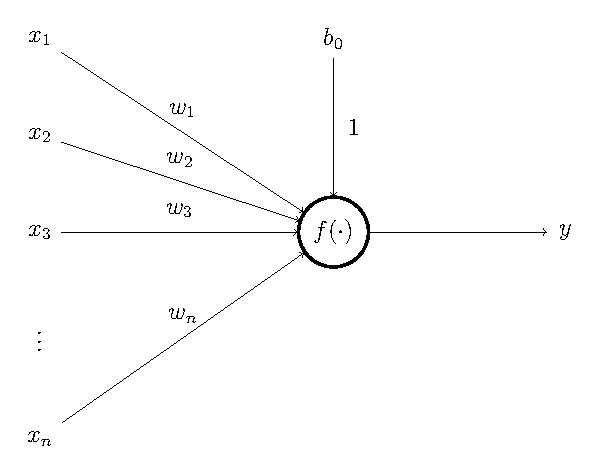
\includegraphics[width=0.9\linewidth]{figures/neuron.eps}
		\caption{Neural Network Node}
		\label{fig:modelNeuron_a}
	\end{subfigure}
	\begin{subfigure}{0.5\linewidth}
		\centering
		\includegraphics[width=0.9\linewidth]{figures/multipolarNeuron.png}
		\caption{Biological Neuron Diagram}
		\label{fig:modelNeuron_b}
	\end{subfigure}
		
	\caption{In Figure~\ref{fig:modelNeuron_a}. each input feature $x_i$ is weighted by its corresponding weight $w_i$. During the training procedure, these weights are adjusted so that the output $y$ approaches the target value. In Figure~\ref{fig:modelNeuron_b}, we see the diagram of an actual multi polar neuron. The dendrites, where the stimuli are received, plays a role similar to that of the input nodes. The axon transmits the signal to the synaptic terminals, that are similar to the $y$ output}
	\label{fig:modelNeuron}
\end{figure}


As far as the activation function is concerned, we can have several types. An immediate choice would be the \textbf{Binary Step Function} that  outputs -1 if the activation is \textbf{below} a given threshold and 1 otherwise. There can also be \textbf{real valued activation functions}, whose output is not binary, but rather that of a continuously differentiable function, such as the logistic sigmoid $\sigma(a) = \frac{1}{1 + \mathrm{e}^{-a}}$ or the hyperbolic tangent $\tanh(a)$. This aspect will prove useful for the usual training methods, that involve the computation of derivatives. In Figure~\ref{fig:activFunc} these activation functions are plotted.

\begin{figure}[H]
	\centering
	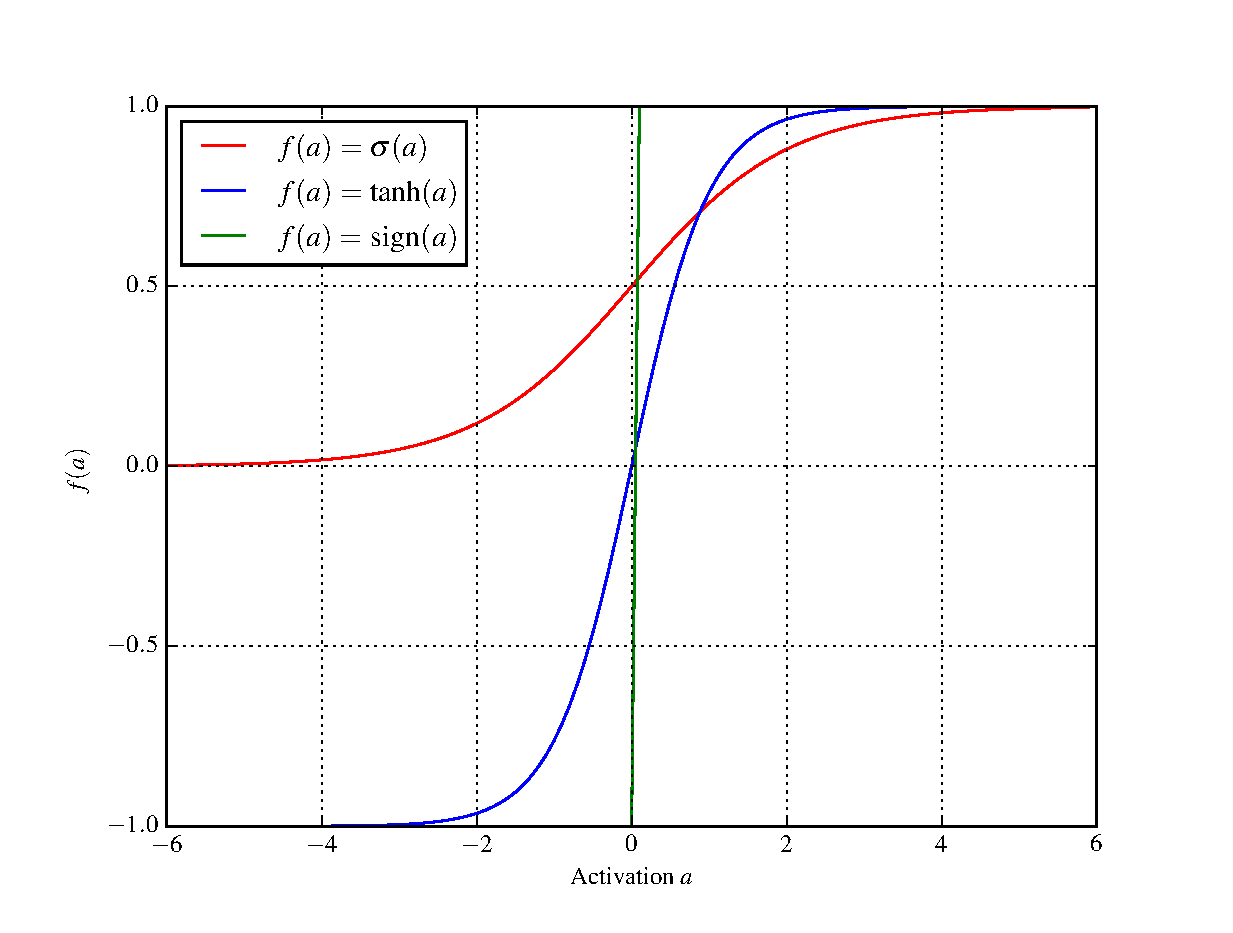
\includegraphics[width=0.9\linewidth]{figures/activFunc.eps}
	\caption{Three different activation functions. As you can see, the hyperbolic tangent has the same extreme value as the sign step function, but has a smooth transition between them, which can be interpreted as a \emph{soft decision} in the more ambiguous middle region, reflecting the degree of uncertainty on the decision. On the other hand, the sigmoid function goes from zero to one, and is also smooth like the hyperbolic tangent}.
	\label{fig:activFunc}
\end{figure}


A neuron by itself can be thought of as a simple linear regression, where we optimize the weight of each feature according to a target value, or function. While important in some applications, the main interest in ANN is to evaluate increasingly more complex models, and not a simple linear regression. This is achieved by \emph{chaining} nodes to one another, connecting the output of a given node to one of the inputs of another. We call \emph{layers} to a group of these nodes that occupy the same hierarchical position. There can be any number of layers, with any number of nodes, but most implementations generally have 3 layers: the \emph{initial} layer, the \emph{hidden} layer (in the middle) and the \emph{output} layer. Figure~\ref{fig:neuralnet} suggests a possible structure for a 3 layer ANN. 


\begin{figure}[H]
	\centering
	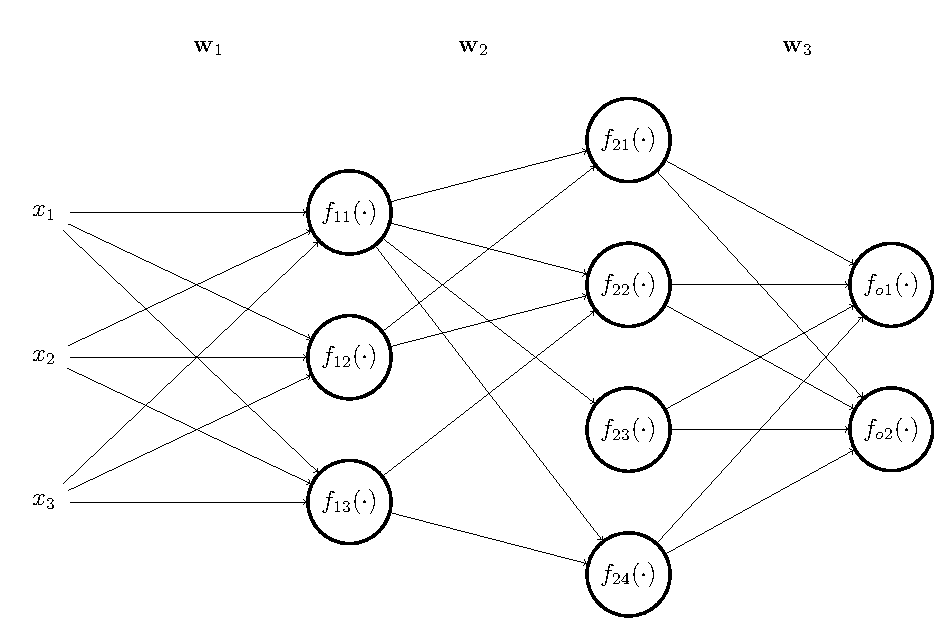
\includegraphics[width=0.9\linewidth]{figures/ann.eps}
	\caption{A three layer ANN. We have omitted some of the connections in the hidden layer, for simplification purposes. $\mb{w}_1$ represents the weight matrix of the input layer, $\mb{w}_2$ the weight matrix of the connections between the input layer and the hidden layer, and $\mb{w}_3$ the weight connections between the hidden and the output layer. $f_{ij}(\dots)$ is the activation function of the $j$-th neuron of the $i$-th layer. Since they can be different, I chose different indexes to each.}
	\label{fig:neuralnet}
\end{figure}

Regarding the training of ANNs, is is performed through a two-step process: first, a \textbf{feed-forward} step where the input is applied, and the activations are evaluated in succession up to the output neurons; then, the perform the \textbf{backpropagation} step, where we calculate the errors in each of the nodes, but now from the output to the input: the weights are updated and optimized using an iterative  method called \textit{Gradient Descent}, where if $\tau$ is the current time step, the next update on the weight matrix $\mb{w}^{(\tau+1)}$ is given by

\begin{equation}\label{eq:gradDesc}
	\mb{w}^{(\tau+1)} = \mb{w}^{(\tau)} - \eta \nabla E(\mb{w}^{(\tau)})
\end{equation}
where $E(\cdot)$ is the error function. As we can see, the weight matrix is moved in the direction that minimizes the error function the most, and $\eta$ controls how fast this is achieved, being the reason why it is called the \textbf{learning rate}.

The computation of gradient of the error function comprises the evaluation of its derivatives with respect to each weight of all network connections, $w_{ij}$. They are

\begin{equation}\label{eq:partialE}
	\frac{\partial E}{\partial w_{ji}} = \delta_j f(a_i)
\end{equation}
where $f(\cdot)$ is the activation function of the neuron and

\begin{equation}\label{eq:deltaj}
	\delta_j = f'(a_j) \sum_k w_{kj} \delta_k .
\end{equation}
The interpretation of these equations is simple. If $w_{ji}$ is the weight of the connection between the neuron $j$ we are considering and a neuron $i$ in a previous layer, then the sum over $k$ relates to all the neurons in the \emph{next} layer to which $j$ connects: this way, since the update on $w_{ji}$, according to~\ref{eq:gradDesc}, is given by

\begin{equation}\label{eq:update}
	w_{ji}^{(\tau+1)} = w_{ji}^{(\tau+1)} - \eta \frac{\partial E}{w_{ji}}
\end{equation}
we see that, from~\ref{eq:partialE}  it simply is the product of the error of the current neuron, $\delta_j$, with the output of the previous neuron $f(a_i)$. In turn, from~\ref{eq:deltaj}, we see the recurrence relationship between it and the weighted sum of all posterior neurons that connect to it. Hence, the name backpropagation is now clear: we are, in fact, propagating the errors backwards into the neuron of interest, weighted by the corresponding weight, but now \emph{backwards} instead of forward, as before. For the output units, the $\delta_j$ is simply the difference between the produced output and the corresponding label for that sample. This two-step process is performed for every data point in out dataset. %%Place where I can include an algorithmic overview?
For a complete proof of the above formulas, see~\citep[chap. 5.3.1]{Bishop2006}.

\section{Recurrent Neural Networks}\label{sec:theorBack_rnn}
A Recurrent Neural Network (RNN) is, essentially, a regular ANN where some neurons (especially in the hidden layer) have \emph{feedback connections} to themselves, i.e. their outputs are fed as inputs. The relevance of this different structure is the possibility to retain \emph{sequence} information about the data. Before, each incoming data point only contributed to the training of the network, but no information about the correlation between themselves and the data points that preceded them did not influence the training step. They were regarded as if no temporal relationship existed, and therefore each data point is conditionally independent of any other. This is obviously not necessarily truth, and in fact there are many cases, where the correlation between data points is high for those closely spaced in time, in which it is actually completely false, as in video signals, audio signals, or other kinds of \emph{temporal sequences} of data. Therefore, the feedback connection of the neuron to himself acts as a kind of \emph{memory element} that takes into account in the present decision, the history of decisions previously taken, and hence the previous data. 
Figure~\ref{fig:recneuron} suggests a possible structure for a neuron of a hidden layer in an RNN, and also an alternate representation, where the structure is unfold through time.

%% METE AQUI A FIGURA

FALAR EM BPTT

Even though RNNs outperform static ANNs in sequence recognition problems~\citep{Bengio1991}, they fail to retain long-term dependencies. Of course that the weight training process is itself a form of memory, but the problem is that the weight update is much slower than the activations~\citep{Yoshua01}, and therefore this memory only retains short-term dependencies. This is because of the so-called \textbf{Vanishing Gradients Problem}~\citep{Yoshua94,Yoshua01}, where the error decays exponentially through time, and the impact of previous incoming data points on the training of the weights quickly decrease. 

To overcome this issue, Hochreiter and Schmidhüber proposed, in 1997, a novel approach, called the Long-Short Term Network~\citep{Hoch97}. The next section explains the main structure of this approach, and also how it is trained, serving as a support basis for the work of this thesis.

\section{Long Short-Term Memory Networks}\label{sec:theorBack_lstm}


